%!TEX root = ../thesis.tex

\subsection{ポテンシャル法}

\begin{figure}[H]
  \centering
 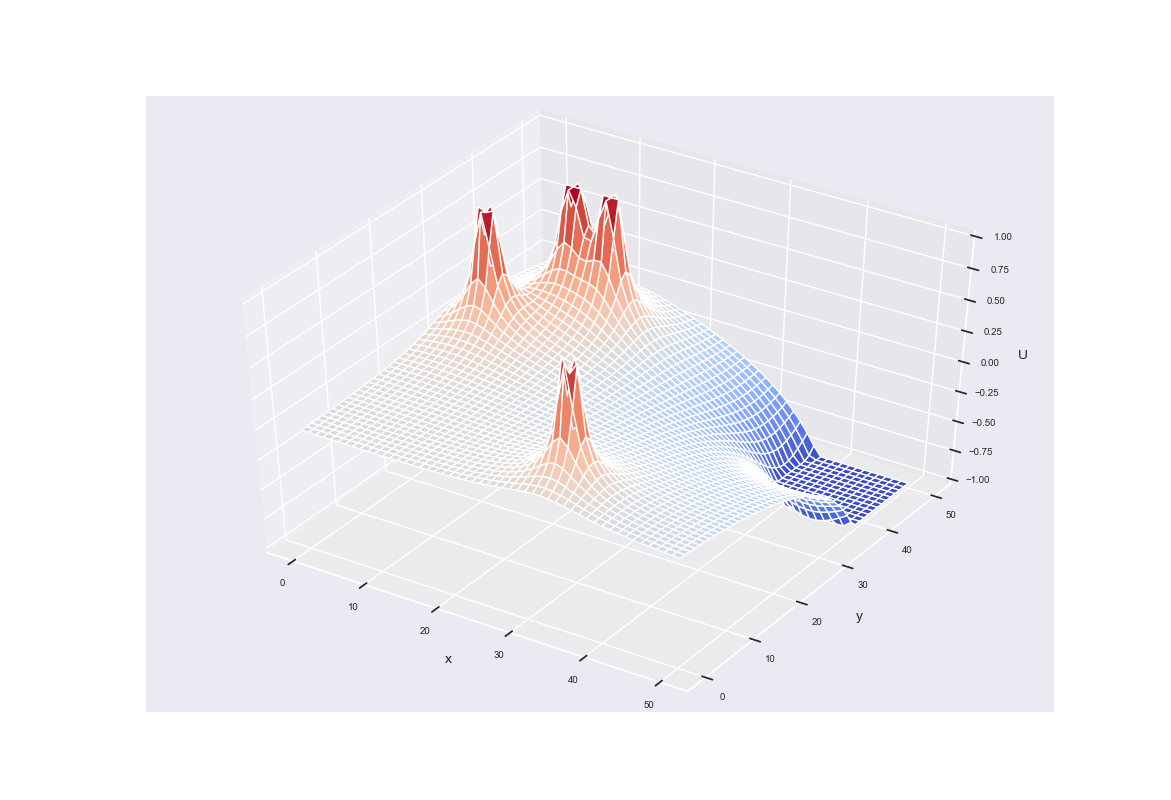
\includegraphics[keepaspectratio, scale=0.4]
      {images/png/potential.png}
 \caption{Potential field ~\cite{pathpt1:online}}
 \label{Fig:potential}
\end{figure}

ポテンシャル法は人工的に作り出したポテンシャル場を使用して,
スタートからゴールまでボールが転がる方向にロボットを移動させる方法である.
ポテンシャル場はゴールが谷底の斜面になっており,障害物は山になる.
スタートからボールを転がすと山と山の間の谷をコロコロと
谷底のゴールに向かって転がっていくというのがポテンシャル法のイメージである.

問題点としては,局所解であるローカルミニマムに陥ってしまうことが挙げられる.
これはゴールではない部分に谷底がもう一つできてしまう現象である.
このローカルミニマムを回避する方法は右手法など様々に研究されている.


\newpage
